\documentclass[aspectratio=169]{beamer}

\usetheme{metropolis}           % Use metropolis theme
\usepackage[utf8]{inputenc}
\usepackage{graphicx}
\usepackage{eso-pic}
\usepackage{graphics}
\usepackage{tikz}
\usepackage[export]{adjustbox}
\usepackage{multicol}
\usepackage{listings}
\usepackage{helvet}
\usepackage{booktabs}
\usepackage{threeparttable}
\usepackage{marvosym}
\usepackage{hyperref}
\usepackage{soul}	% For strike-through
\usepackage{tcolorbox} % For color box
\usepackage{url}

\title{Introduction to Python\\for Stata Users}
\date{}
\author{Luis Eduardo San Martin} % Name of author(s) of session here
\institute{Development Impact Evaluation (DIME) \newline The World Bank }
\setbeamercolor{background canvas}{bg=white}	% Sets background color

% The below command places the World Bank logo and DIME logo to the right corner
\titlegraphic{%
	\begin{picture}(0,0)
	\put(330,-180){\makebox(0,0)[rt]{
\includegraphics[width=3cm]{img/WB_logo}}}
	\end{picture}%
	\begin{picture}(0,0)
	\put(390,-180){\makebox(0,0)[rt]{
\includegraphics[width=1.5cm]{img/i2i}}}
	\end{picture}%
}

%%% Section page with picture of Light bulb
\makeatletter
\defbeamertemplate*{section page}{mytheme}[1][]{
	\centering
	\begin{minipage}{22em}
		\raggedright
		\usebeamercolor[fg]{section title}
		\usebeamerfont{section title}
		\par
		\ifx\insertsubsectionhead\@empty\else%
		\usebeamercolor[fg]{subsection title}%
		\usebeamerfont{subsection title}%
		\fi
		\ifstrempty{#1}{}{%
			\includegraphics[width=100mm, height=60mm]{#1}%
		}
		\\
		\insertsectionhead\\[-1ex]
		\insertsubsectionhead
		\usebeamertemplate*{progress bar in section page}
		
	\end{minipage}
	\par
	\vspace{\baselineskip}
}
\makeatother

%%% Define a command to include picture in section, 
%%% make section, and revert to old template
\newcommand{\sectionpic}[2]{
	\setbeamertemplate{section page}[mytheme][#2]
	\section{#1}
	\setbeamertemplate{section page}[mytheme]
}

%%% The command below allows for the text that contains Stata code
\lstset{ %
	backgroundcolor=\color{white},
	basicstyle=\tiny,
	breakatwhitespace=false,
	breaklines=true,
	captionpos=b,
	commentstyle=\color{green},
	escapeinside={\%*}{*)},
	extendedchars=true,
	frame=single,
	numbers=left,
	numbersep=5pt,
	numberstyle=\tiny\color{gray},
	rulecolor=\color{black},
	showspaces=false,
	showstringspaces=false,
	showtabs=false,
	stringstyle=\color{mauve},
	tabsize=2,
	title=\lstname,
	morekeywords={not,\},\{,preconditions,effects },
	deletekeywords={time}
}

%% The below command creates the ligh bulb logos in the top right corner of the 
\begin{document}
	
	
	%%%%%%%%%%%%%%%%%%%%%%%%%%%%%%%%%%%%%%%%%%% Title slide
	{
		\usebackgroundtemplate{
\includegraphics[height=55mm,right]{img/top_right_corner.pdf}} 
		\maketitle
	}

\begin{frame}

	\frametitle{Overview} % Table of contents slide, comment this block out to remove it
	\tableofcontents % Throughout your presentation, if you choose to use \section{} and \subsection{} commands, these will automatically be printed on this slide as an overview of your presentation

\end{frame}

%%%%%%%%%%%%%%%%%%%%%%%%%%%%%%%%%%%%%%%%%%% Section title slide
\sectionpic{Web scraping overview}{img/section_slide}

%%%%%%%%%%%%%%%%%%%%%%%%%%%%%%%%%%%%%%%%%%% Regular slides
\begin{frame}{Web scraping overview}

	\begin{itemize}
		\item For this second part of the session, we'll do a web scraping exercise
		\item We'll transform the table shown in this URL: \url{https://datatables.net/examples/basic_init/zero_configuration.html} into a csv file
	\end{itemize}

\end{frame}

\begin{frame}{Web scraping overview}

	Before starting, we'll give a bit more context on web scraping	

	\begin{itemize}
		\item You'll probably know that every website you visit has an underlying \texttt{html} code
		\item A simple example:
	\end{itemize}

	\begin{multicols}{2}

		\begin{figure}
			\centering
			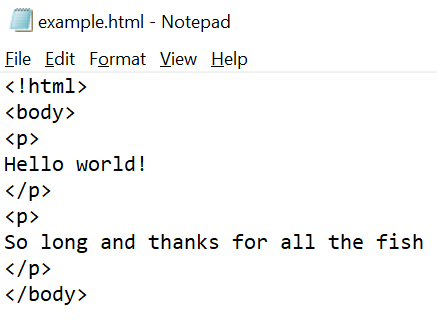
\includegraphics[width=0.7\linewidth]{img/html_example.png}
		\end{figure}
		\begin{figure}
			\centering
			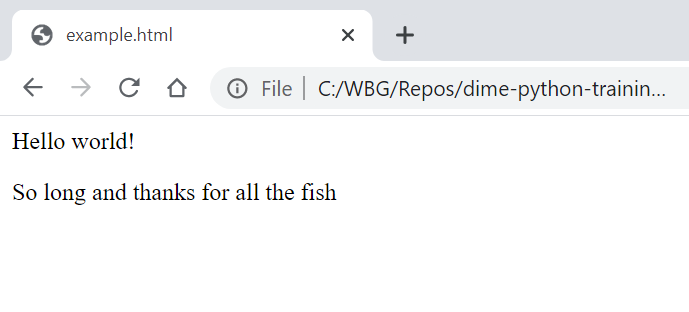
\includegraphics[width=\linewidth]{img/html_example_rendered.png}
		\end{figure}

	\end{multicols}

	\begin{itemize}
		\item Your web browser renders this code and shows you the result 
	\end{itemize}

\end{frame}

\begin{frame}{Web scraping overview}

	When performing web scraping, we're basically doing two operations

	\begin{enumerate}
		\item We retrieve the underlying raw \texttt{html} code of a website
	\end{enumerate}

	\begin{multicols}{2}

		\begin{figure}
			\centering
			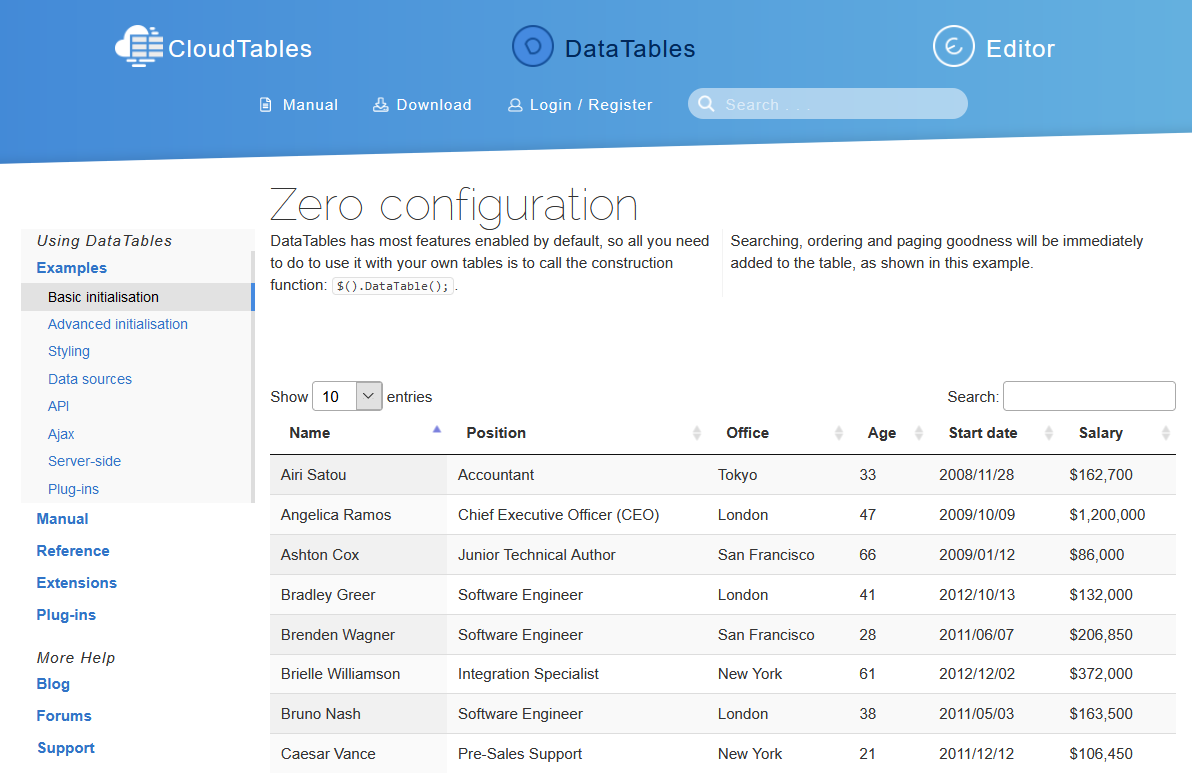
\includegraphics[width=0.7\linewidth]{img/website_example.png}
		\end{figure}
		\begin{figure}
			\centering
			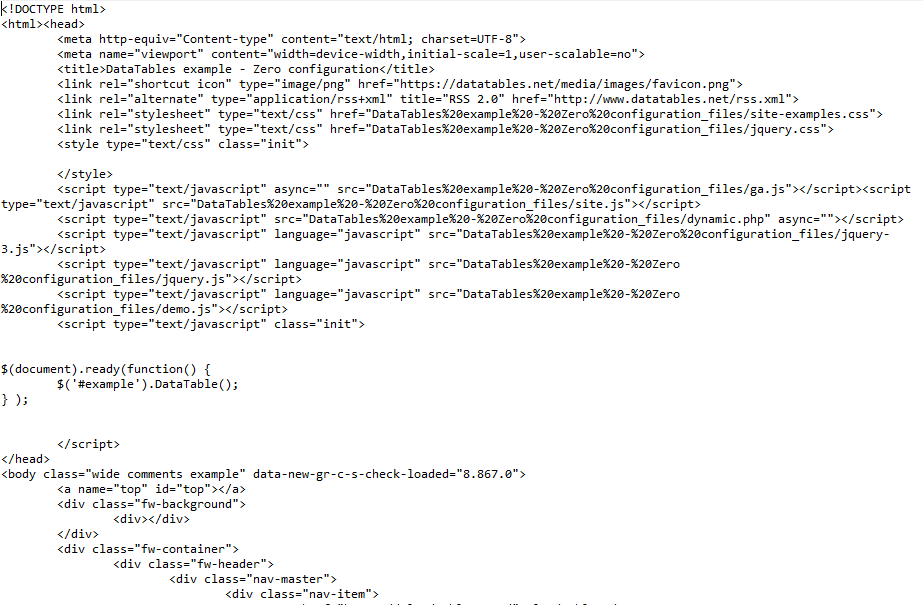
\includegraphics[width=\linewidth]{img/website_example_html.png}
		\end{figure}

	\end{multicols}

\end{frame}

\begin{frame}{Web scraping overview}

	2. From the raw \texttt{html} code, we locate the part that is relevant for us to extract and arrange it into an variable we can use

	\begin{multicols}{2}

		\begin{figure}
			\centering
			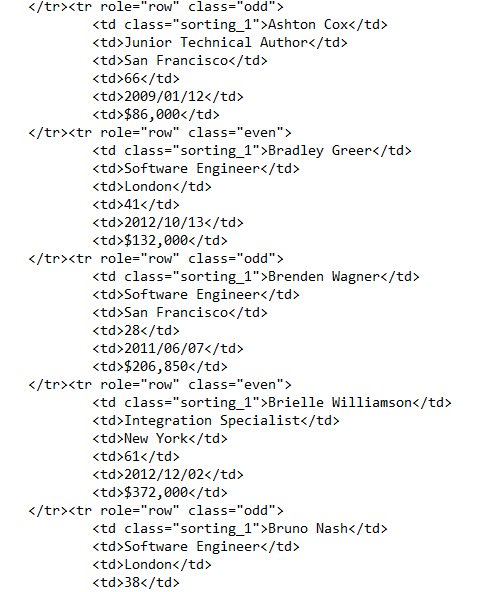
\includegraphics[width=0.7\linewidth]{img/html_relevant.png}
		\end{figure}
		\begin{figure}
			\centering
			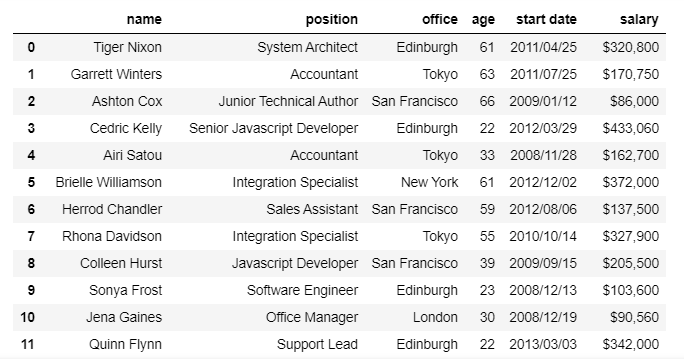
\includegraphics[width=\linewidth]{img/html_final.png}
		\end{figure}

	\end{multicols}

\end{frame}

\begin{frame}{Web scraping overview}

	\begin{itemize}	
		\item To execute these operations, we'll need to use three Python libraries.
		\item Libraries are similar to the user-written Stata commands you download from the \texttt{ssc} repository, except that you have to manually load them in each new Python session you start.
		\item Each library has custom made data types with operations specific to the topic of the library.
		\item To install libraries, we would normally have to use Window's or Mac's command lines. However, we'll skip installing for now because Colab has the libraries we need already pre-installed.
	\end{itemize}

\end{frame}

\begin{frame}{Web scraping overview}

	To load libraries, we use \texttt{import}

	\begin{figure}
		\centering
		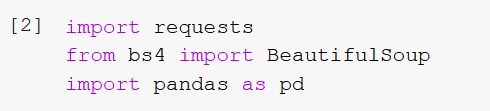
\includegraphics[width=0.4\linewidth]{img/libraries.png}
	\end{figure}

	\begin{itemize}
		\item \texttt{requests} is an \texttt{html} requestor. We'll use it to retrieve the \texttt{html} code of our URL
		\item \texttt{BeautifulSoup} is a text parser. We'll use it to extract the information we need from the \texttt{html} code
		\item \texttt{pandas} is a dataframe manipulation library. We'll use to structure the information into a dataframe and export the result to a \texttt{csv} file
	\end{itemize}

\end{frame}

%%%%%%%%%%%%%%%%%%%%%%%%%%%%%%%%%%%%%%%%%%% Section title slide
\sectionpic{Web scraping - Retrieving raw \texttt{html} code}{img/section_slide}

%%%%%%%%%%%%%%%%%%%%%%%%%%%%%%%%%%%%%%%%%%% Regular slides
\begin{frame}{Web scraping - Retrieving raw \texttt{html} code}

	We'll use the command \texttt{get()} from \texttt{requests} to retrieve the \texttt{html} code. We'll start by saving the result of the request in an variable called \texttt{response}

	\begin{figure}
		\centering
		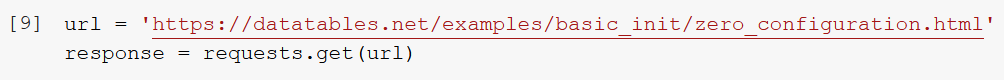
\includegraphics[width=\linewidth]{img/response.png}
	\end{figure}

\end{frame}

\begin{frame}{Web scraping - Retrieving raw \texttt{html} code}

	\texttt{response} is a data type that contains not only the \texttt{html} code we're looking for, but also information about our html request itself. For example, we can use \texttt{status\_code} to check if our request was successful:

	\begin{figure}
		\centering
		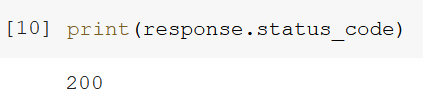
\includegraphics[width=0.4\linewidth]{img/status_code.png}
	\end{figure}

	A value of \texttt{200} indicates that the request worked

\end{frame}

\begin{frame}{Web scraping - Retrieving raw \texttt{html} code}

	After we checked that the request was successful, 
	we use an attribute called \texttt{.text} on the response data type 
	to extract the html code from the page we requested. 
	The result is a single very long string.

	\begin{figure}
		\centering
		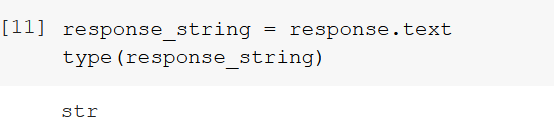
\includegraphics[width=0.4\linewidth]{img/response_string.png}
	\end{figure}

	\texttt{response\_string} contains the raw \texttt{html} code we need

\end{frame}

%%%%%%%%%%%%%%%%%%%%%%%%%%%%%%%%%%%%%%%%%%% Section title slide
\sectionpic{Web scraping - Extracting and arranging information}{img/section_slide}

%%%%%%%%%%%%%%%%%%%%%%%%%%%%%%%%%%%%%%%%%%% Regular slides
\begin{frame}{Web scraping - Extracting and arranging information}

	Now we need to manually explore the \texttt{html} string and locate the information of interest. We can use \texttt{print()} for this

	\begin{figure}
		\centering
		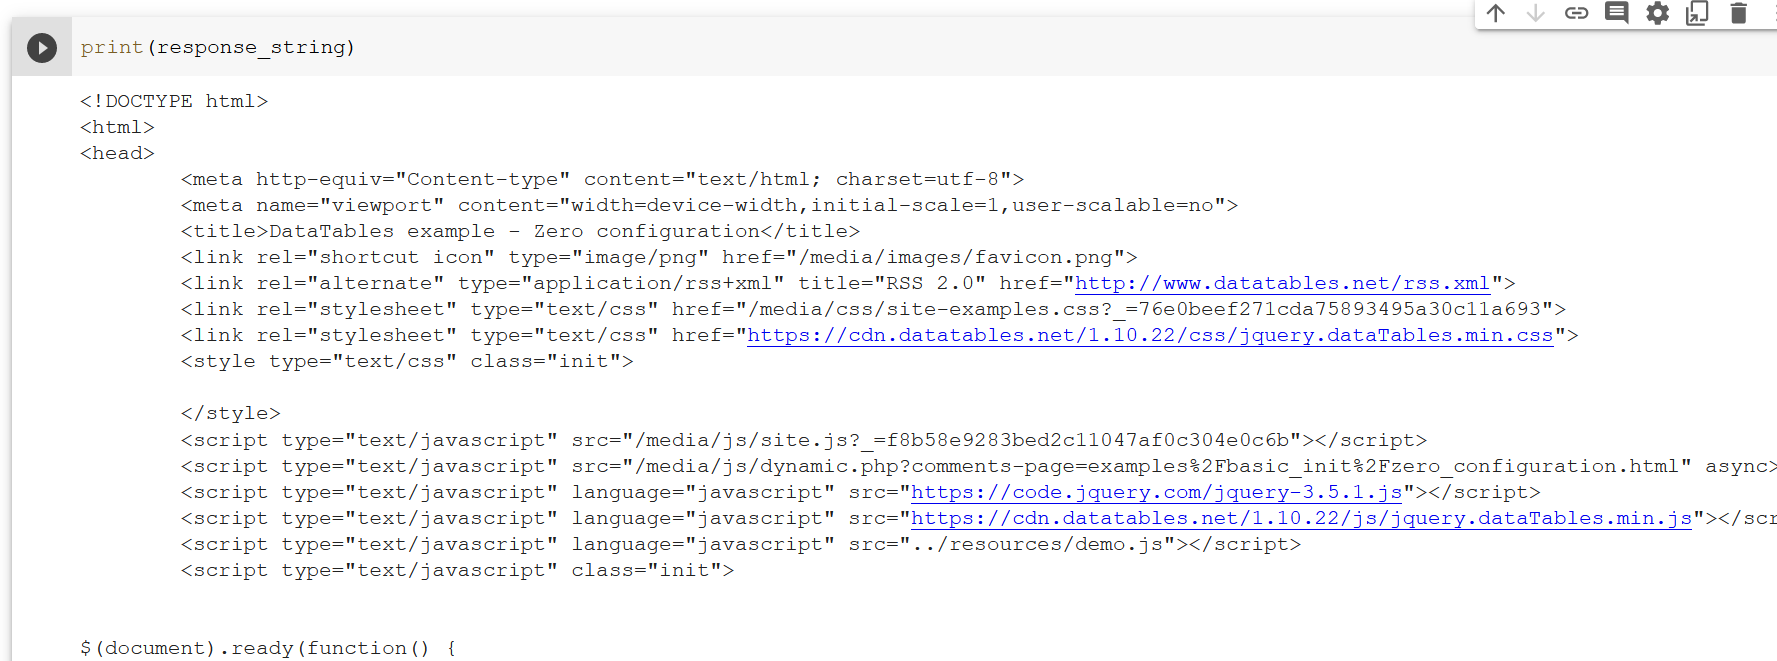
\includegraphics[width=0.9\linewidth]{img/html_string_print.png}
	\end{figure}

\end{frame}

\begin{frame}{Web scraping - Extracting and arranging information}

	This manual inspection allow us to see that every single observation in our target table is enclosed between \texttt{tr} tags, and that every piece of information inside an observation is enclosed in \texttt{td} tags
	
	\begin{columns}[c]
		\column{.50\textwidth} % Left column and width

		\begin{figure}
			\centering
			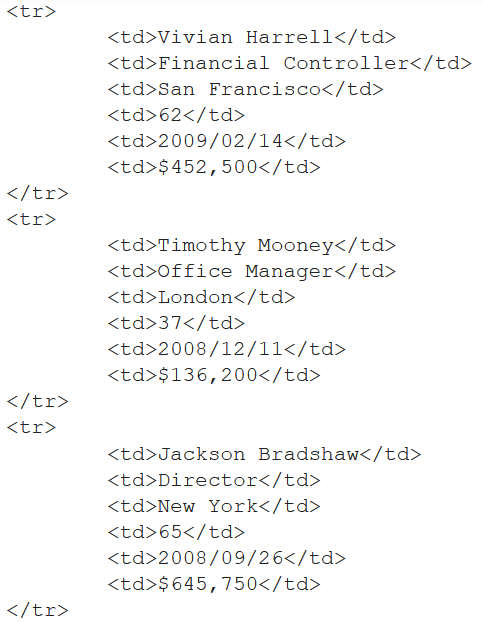
\includegraphics[width=0.6\linewidth]{img/tags2.png}
		\end{figure}
		
		\column{.50\textwidth} % Right column and width
		\begin{itemize}
			\item \texttt{tr} - stands for "table row"
			\item \texttt{td} - stands for "table data cell"
		\end{itemize}
		
	\end{columns}


\end{frame}

\begin{frame}{Web scraping - Extracting and arranging information}

	Then, we need to do the following:

	\begin{enumerate}
		\item From the whole string, extract every content enclosed in \texttt{tr} tags
		\item For each of the contents enclosed in \texttt{tr} tags, extract every piece of information enclosed in \texttt{td} tags
	\end{enumerate}

	We'll use \texttt{BeautifulSoup} for this 
	- a commonly used library to extract information from an html code

\end{frame}

\begin{frame}{Web scraping - Extracting and arranging information}

	\begin{itemize}	
		\item \texttt{BeautifulSoup} parses a string by detecting symbols and spacing that creates sections and subsections in plain text
		\item If used in \texttt{html} code, it knows automatically that tags are used to specify sections
	\end{itemize}

\end{frame}

\begin{frame}{Web scraping - Extracting and arranging information}

	\begin{itemize}
		\item To parse an \texttt{html} string, we use the following code:
	\end{itemize}

	\begin{figure}
		\centering
		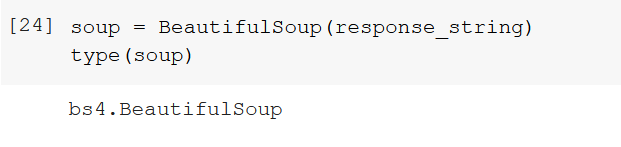
\includegraphics[width=0.7\linewidth]{img/bs4_type.png}
	\end{figure}

	\begin{itemize}	
		\item The result is not a string anymore, but a \texttt{BeautifulSoup} data type
		\item You can think of it as a text with divisions and subdivisions with many operations to work with the content
	\end{itemize}

\end{frame}

\begin{frame}{Web scraping - Extracting and arranging information}

	\begin{multicols}{2}

		\begin{itemize}
			\item The advantage of using this type as opposed to a string is that now we can directly look for any divisions enclosed by the the \texttt{tr} tags
			\item We'll use the \texttt{.find\_all()} attribute for this and save the result in a new variable named \texttt{observations}
			\item Note that \texttt{observations} is a list
		\end{itemize}

		\begin{figure}
			\centering
			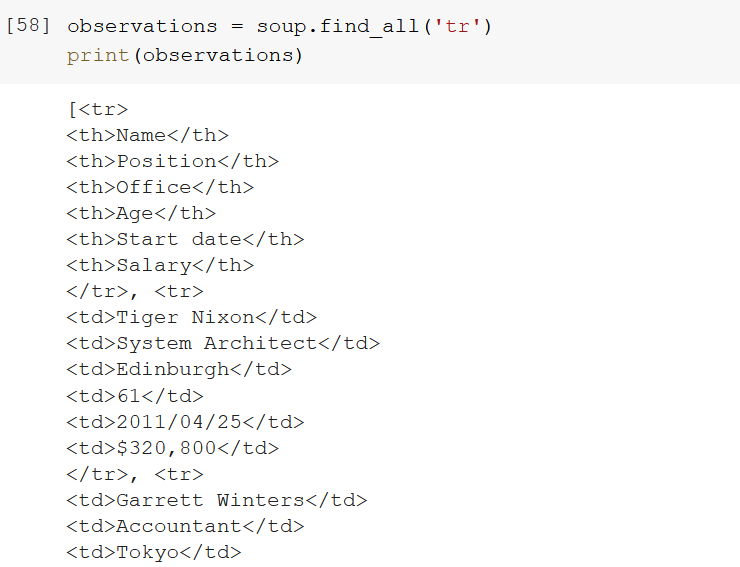
\includegraphics[width=\linewidth]{img/tr_list.png}
		\end{figure}
	
	\end{multicols}

\end{frame}

\begin{frame}{Web scraping - Extracting and arranging information}

	\begin{itemize}
		\item \texttt{observations} is a list that contains every piece of text that was enclosed in \texttt{tr} tags, including the tags themselves
		\item Nonetheless, every element of it is not a string, but another \texttt{BeautifulSoup} data type
		\item If we inspect a single element of \texttt{observations}, we get this:
	\end{itemize}

	\begin{figure}
		\centering
		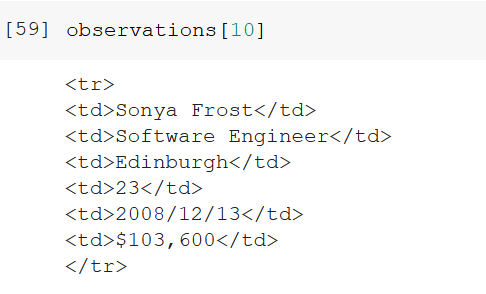
\includegraphics[width=0.5\linewidth]{img/tr_list_element.png}
	\end{figure}

\end{frame}

\begin{frame}{Web scraping - Extracting and arranging information}

	\begin{itemize}
		\item You might see by now that we're getting closer to our final result!
		\item We basically need to iterate through the elements of \texttt{observations} and extract everything that is inside the \texttt{td} tags
		\item Since the elements of \texttt{observations} are still \texttt{Beautiful Soup} data types, we can use once again the \texttt{.find\_all()} attribute for this 
	\end{itemize}

\end{frame}

\begin{frame}{Web scraping - Extracting and arranging information}

	\begin{itemize}
		\item For a single element, this would be:
	\end{itemize}

	\begin{figure}
		\centering
		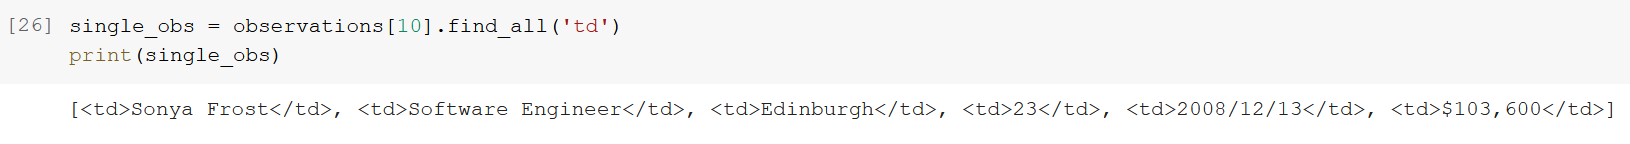
\includegraphics[width=1.02\linewidth]{img/td_list.png}
	\end{figure}

	\begin{itemize}
		\item This is \textit{almost} what we want, except that it still includes the \texttt{td} tags
	\end{itemize}

\end{frame}

\begin{frame}{Web scraping - Extracting and arranging information}

	To eliminate them, we need to use \texttt{.text} with every element of \texttt{single\_obs}

	\begin{figure}
		\centering
		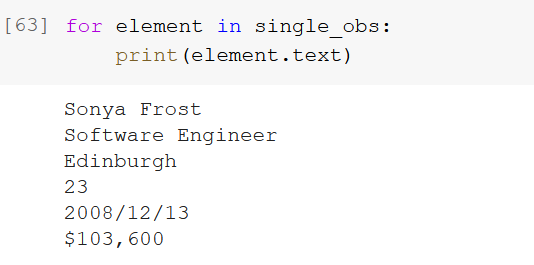
\includegraphics[width=0.5\linewidth]{img/td_list_text.png}
	\end{figure}

	Now every one of these is a string data type again!

\end{frame}

\begin{frame}{Web scraping - Extracting and arranging information}

	Furthermore, we can modify this code to save the result in a new list

	\begin{figure}
		\centering
		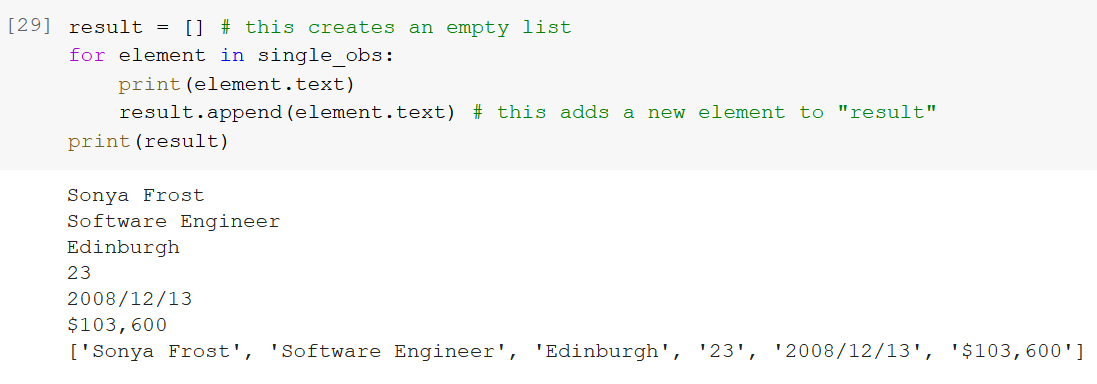
\includegraphics[width=0.9\linewidth]{img/td_new_list_text.png}
	\end{figure}

\end{frame}

\begin{frame}{Web scraping - Extracting and arranging information}

	Now that we finally figured out how to extract the information we want, we just need to loop over \texttt{observations} to generalize our approach and get the entire information

	\begin{figure}
		\centering
		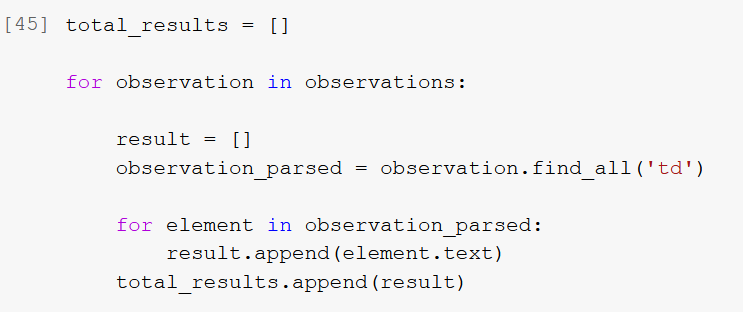
\includegraphics[width=0.6\linewidth]{img/tr_loop.png}
	\end{figure}

\end{frame}

\begin{frame}{Web scraping - Extracting and arranging information}

	\begin{itemize}	
		\item You might have noticed that the first and last elements of \texttt{total\_results} are empty lists
		\item This is because in our original \texttt{html} string, the first and last elements enclosed in \texttt{tr} tags didn't contain any elements enclosed in \texttt{td} tags. Then, using \texttt{observation.find\_all("td")} produced an empty lists in both cases
		\item We can easily eliminate these observations from \texttt{total\_results} by subsetting the list and excluding the last and first elements
	\end{itemize}

	\begin{figure}
		\centering
		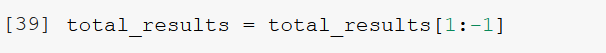
\includegraphics[width=0.6\linewidth]{img/total_results_subsetting.png}
	\end{figure}

\end{frame}

\begin{frame}{Web scraping - Extracting and arranging information}

	\begin{itemize}
		\item \texttt{total\_results} contains the result we wanted to have. Great!
		\item The final step is to export it to a \texttt{csv} file
		\item Remember that we loaded the \texttt{pandas} library? We'll use it now
	\end{itemize}

\end{frame}

\begin{frame}{Web scraping - Extracting and arranging information}

	First, we create a \texttt{pandas} dataframe where we insert \texttt{total\_results} as data. We call the dataframe \texttt{df}

	\begin{figure}
		\centering
		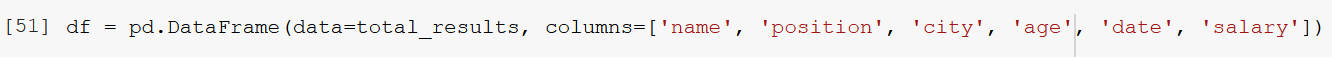
\includegraphics[width=\linewidth]{img/df.png}
	\end{figure}

	\texttt{pd.DataFrame()} uses two arguments in this case:

	\begin{enumerate}
		\item \texttt{data}: the data we're loading to the dataframe
		\item \texttt{columns}: a list of strings with the column names
	\end{enumerate}

	Pandas dataframes are a data type that is similar to a dataset in Stata

\end{frame}

\begin{frame}{Web scraping - Extracting and arranging information}

	\begin{figure}
		\centering
		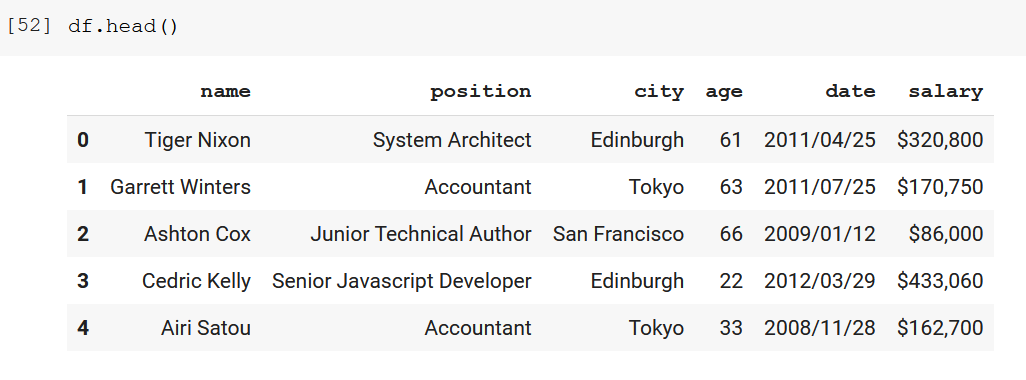
\includegraphics[width=\linewidth]{img/df_head.png}
	\end{figure}

\end{frame}

\begin{frame}{Web scraping - Extracting and arranging information}

	Finally, we export \texttt{df} into a \texttt{csv} file using the attribute \texttt{.to\_csv()}

	\begin{figure}
		\centering
		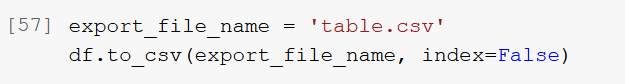
\includegraphics[width=0.6\linewidth]{img/df_to_csv.png}
	\end{figure}

	\texttt{pandas} by default exports a column with the index numbers. We use \texttt{index=False} to omit it 

\end{frame}

\begin{frame}{Web scraping - Extracting and arranging information}

	\begin{itemize}
		\item Since we were using Colab in this exercise, we just exported \texttt{table.csv} to the cloud
		\item To download the result to your computer, click the folder icon to the left, locate your file, click on the vertical ellipsis next to it and click \texttt{Download}
	\end{itemize}

	\begin{figure}
		\centering
		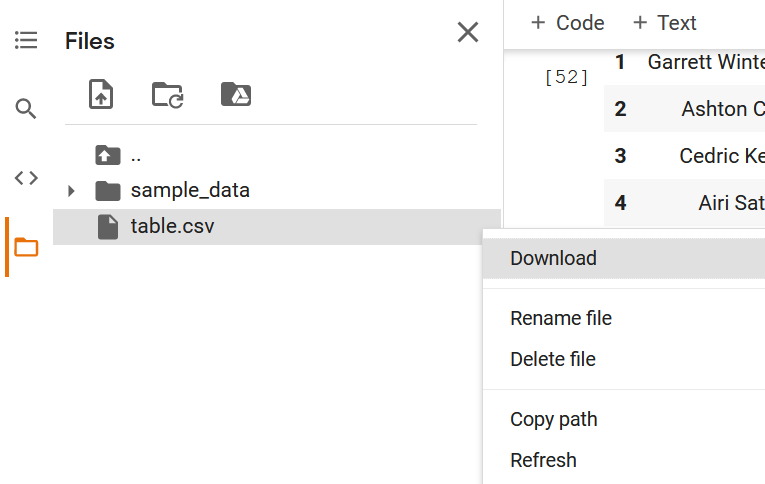
\includegraphics[width=0.5\linewidth]{img/colab_download.png}
	\end{figure}

\end{frame}

\end{document}